%!TEX root = ../thesis.tex
%*******************************************************************************
%*********************************** Sixth Chapter *****************************
%*******************************************************************************

\chapter{Investigation of changes of the basal impedance signal}  %Title of the First Chapter
\label{chapter basal}

\ifpdf
\graphicspath{{Chapter6/Figs/Raster/}{Chapter6/Figs/PDF/}{Chapter6/Figs/}}
\else
\graphicspath{{Chapter6/Figs/Vector/}{Chapter6/Figs/}}
\fi

One of the characteristics of the impedance plethysmography device is the ability to measure the basal impedance of any tissue with a cylindrical shape, in this case, the left forearm. The data collected using the procedure described in chapter \ref{chapter procedure} provided characteristics of the impedance from eight participants. During the whole test, four regions contained information about the baseline impedance either previous or after an upper arm occlusion, which are the regions 1, 3, 5 and 7 of the data sets. 

The results presented in this chapter describe the different elements that may affect the resistive baseline impedance during a measurement. For this, the baseline measurements were extracted from the whole data from the regions previously explained. It must be noticed that the baseline regions consists on \SI{5}{\minute} of recordings either before or after an occlusion. Hence, \SI{2}{\minute} of recovery to baseline were allowed before extracting the data to be analysed. Therefore, during the post-processing, the last three minutes of the baseline signals were gathered and analysed per participant. The information collected shows insights of what noises may affect the measurements and what frequency components alter the baseline signal. 

%%********************************** % Section 6.1 ******************************************
\section{Basal impedance results}
\label{section basal 1}
As it can be seen from the instrument's block diagram (see figure \ref{fig:block}), the iPG device provides an output signal denominated $Z_{DC}$ which is equivalent to the mean impedance value of the elbow to wrist segment. The iPG device was able to detect the forearm's segment impedance quite remarkably. The values obtained fell within the resistive value in the tens Ohms as estimated by the literature \cite{dai2009vivo, faes1999electric, grimnes1983impedance}. This section will describe the elements that affected the baseline impedance of the signal. For this, the data was portioned to the last \SI{3}{\minute} of the recorded baselines. By doing this, the effect of the movement and recovery time of the forearm after releasing the occlusion was diminished. 

It must be remarked that the baseline signal also contains an AC component equivalent to the arterial pulses. For the analysis of this section, the APA information was suppressed. Only, the resistivity mean value also known as basal impedance was computed, which is equivalent to the value of $R_B$ as in Nyober's equation \ref{eq:nyober dV} or the foot of the signal in the plethysmography waveform. In other words, it is the value of the impedance before circulation occurs and is composed of the impedance contribution of bone, muscle, fat, skin and residual blood within the vessels \cite{dai2009vivo}. 

Figure \ref{fig:Basal statistics} shows the statistic values of the median basal impedance during the regions 1, 3, 5 and 7. The mean resistive baseline impedance of all the participants was \SI{78.62(1461)}{\ohm}. The impedance was entirely independent of the person sex.  

\begin{figure}[!htbp]
	\centering
	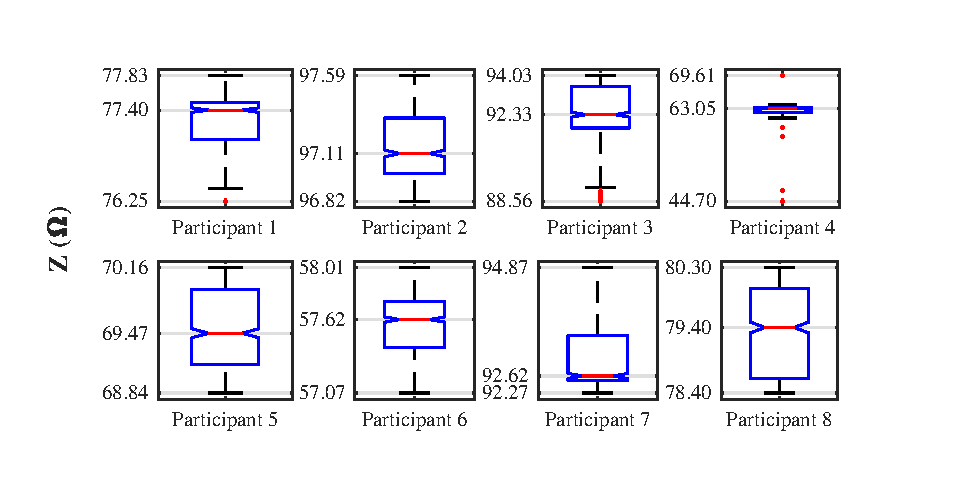
\includegraphics[width=0.85\textwidth,keepaspectratio]{figure_b_1}    
	\caption[Mean basal impedance boxplot]{Mean basal impedance of all the participants during the last \SI{3}{\minute} of the baseline regions 1, 3, 5 and 7.}
	\label{fig:Basal statistics} 
\end{figure}

Artefact motion caused the outliers of the readings. As it can be noticed from the plot, participants 1, 3 and especially 4 presented deviated points during the study. Also, participants 3, 4 and 8 showed the largest distribution between interquartile values larger than \SI{1}{\ohm} (mean \SI{1.41(39)}{\ohm}). The rest of the participants showed a distribution within first and third interquartile of about \SI{0.57(27)}{\ohm}. 

%%********************************** % Section 6.2 ******************************************
\subsection{Relation between geometry and mean basal impedance}
\label{senction basal 2}
There are different aspects of the geometry that could affect the impedance reading. There have been several studies which demonstrated how the distance between electrodes affects readings on tissue \cite{kun2000effects, yamamoto1992impedance}. This study portrayed that he forearm's circumference and the distance between the potential electrodes influences the impedance measurement. Figure \ref{fig:C_vs_Z} indicates that there is an inverse relation between circumference and impedance (slope \SI{-0.072}{\centi\meter\per\ohm}). The smaller the forearm's circumference, the higher the resistivity. On the other hand, there is a direct relation between the distance between the potential electrodes and the resistivity of the segment (slope \SI{0.055}{\centi\meter\per\ohm}) as depicted in \ref{fig:l_vs_Z}.

Moreover, when comparing total volume measured to the mean resistivity of the segment (see figure \ref{fig:Ve_vs_Z}), the impedance tends to increase when the forearm's segment volume decreases (slope \SI{-0.622}{\cubic\centi\metre\per\ohm}). Which is in agreement with the fact that when more tissue is involved in the measurement, the more conductive path for the current, reducing the total impedance. However, this can not be seen as an entirely linear relationship as the impedance value can be affected by the amount of adipose tissue. Having two different arms with same dimensions, the one with more fat will produce a different basal impedance reading that the one with a higher muscular tone. 

\begin{figure*}[!b]
	\centering
	\begin{subfigure}[t]{0.48\textwidth}
		\centering
		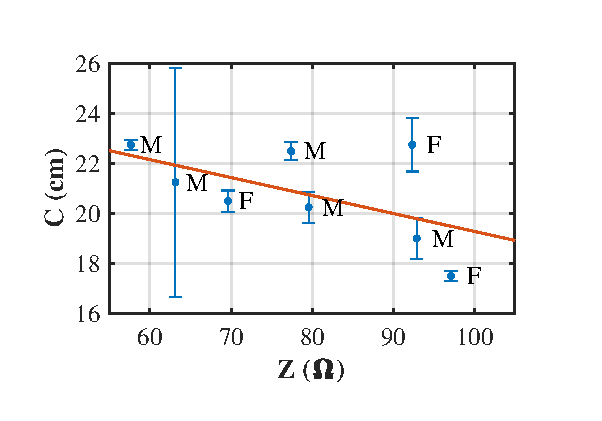
\includegraphics[width=7cm]{figure_b_2a}
		\caption{Relationship between forearm circumference and mean basal impedance}
		\label{fig:C_vs_Z}
	\end{subfigure}%
	~ 
	\begin{subfigure}[t]{0.48\textwidth}
		\centering
		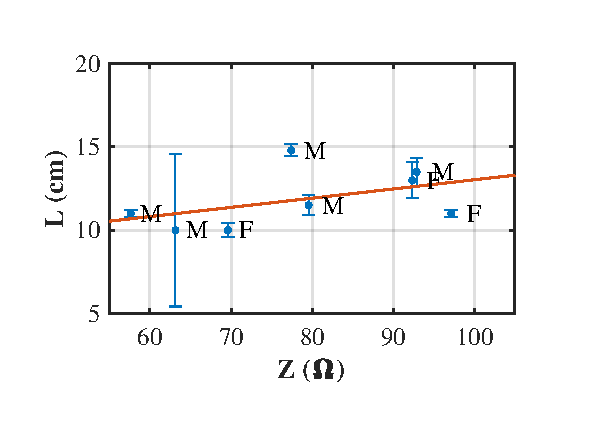
\includegraphics[width=7cm]{figure_b_2b}
		\caption{Relationship between distance sensing electrodes and mean basal impedance}
		\label{fig:l_vs_Z}
	\end{subfigure}
	~ 
	\begin{subfigure}[t]{0.48\textwidth}
		\centering
		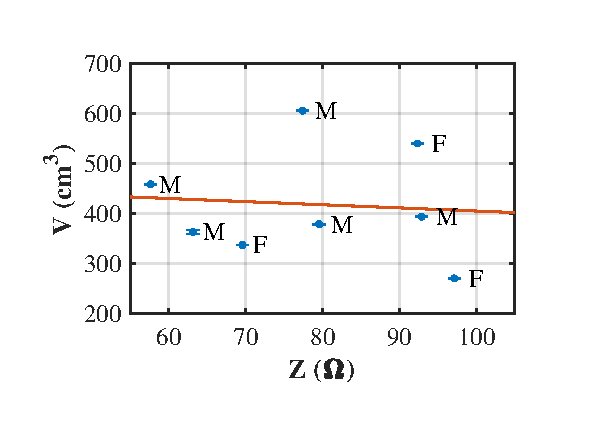
\includegraphics[width=7cm]{figure_b_2c}
		\caption{Relation between forearms segment volume and mean basal resistivity}
		\label{fig:Ve_vs_Z}
	\end{subfigure}
	\caption{Relation between circumference, length and total segment's volume and mean basal impedance}
	\label{fig:relation_geometry_vs_impedance}
\end{figure*}

%%********************************** % Section 6.3 ******************************************
\section{Basal impedance changes between measurements}
\label{senction basal 3}
There are different artefacts that can alter the basal impedance during a measurement such as either motion or respiration movement \cite{pandey2006cancellation, swanson1983errors, ansari2010impedance, rosell1995reduction}. In this section will analysed how much the basal impedance changes between measurements. All the participants were asked to stay still for the whole duration of the test. However, in practice, this is not completely possible as keeping the same position for a prolonged period of time can be quite tiring. Inflating the cuff to a pressure above diastolic level may cause discomfort to the participants like tingling sensation or even pain, a normal response of the body is to move the limb to restore the blood flow. The first \SI{2}{\minute} of the baseline impedance readings may be affected by the rearrange of the participant's position specially after the occlusion of the upper arm. Moreover, the blood flow restriction also induced a physiological response which needed some time to go back to baseline value. Hence, the baseline data after \SI{2}{\minute} is used for this analysis, allowing enough time to recover. 

The data used for the analysis was compiled by extracting the lower envelope of the raw basal impedance. The command envelope in Matlab \cite{MATLAB:2016} allows to isolate the desired signal. Figure \ref{fig:Basal Regions} shows the waveform extracted with the respective mean value for each region per participant. The region 1 applies to the time where the initial reference was recorded, in total \SI{5}{\minute} were recorded but the last \SI{3}{\minute} of data were extracted right before the occlusion between \SIrange{120}{300}{\second}. This basal impedance is the reference to the other readings as was not affected by occlusion of any kind. The other sections of the data correspond to the region 3 which is the recovery after venous occlusion, the information extracted belongs to the time slot between \SIrange{ 600}{780}{\second}.  Similarly, the region 5 after partial arterial occlusion retrieving the last \SI{3}{\minute} of data between \SIrange{1080}{1260}{\second}. Finally, the data after total occlusion in region 7 between \SIrange{1560}{1740}{\second}.

Initially, the first thing that can be observed from the figure is the presence of oscillations in the baseline signal. This signal was present in all the participants with subtle frequency variations between each region. The frequency was calculated by extracting the period of the signal as the difference between its peaks. In average the frequency of the oscillation was \SI{0.0685(00027)}{\hertz}. At this point, it is not possible to establish if this is either a common noise coming from the instrument or a physiological response. In the literature, there is not much information about impedance plethysmographic oscillations at this frequency band.  However, a study using laser Doppler flowmetry found that physiological measurements into this frequency spectrum may be related to the sympathetic activity (\SIrange{0.02}{0.06}{\hertz}) \cite{kvandal2006low}. Further investigation has to be performed to discover the roof of this signal. 

Secondly, it is evident that the motion artefact altered some of the measurements. Participants 3 and 4 clearly displayed deviation from their mean values in region 2 and region 4 respectively. In fact, the figure had to be clipped to fit the waveform information properly. On the other hand, it is hard to detect great changes on partaker 1, but region 3 displayed significant variations compared to the other areas. Hence, this qualitative analysis also confirms the quantitative results showed in figure \ref{fig:Basal statistics}.  

\begin{figure}[!htbp]  %fig:rb:all_participants
	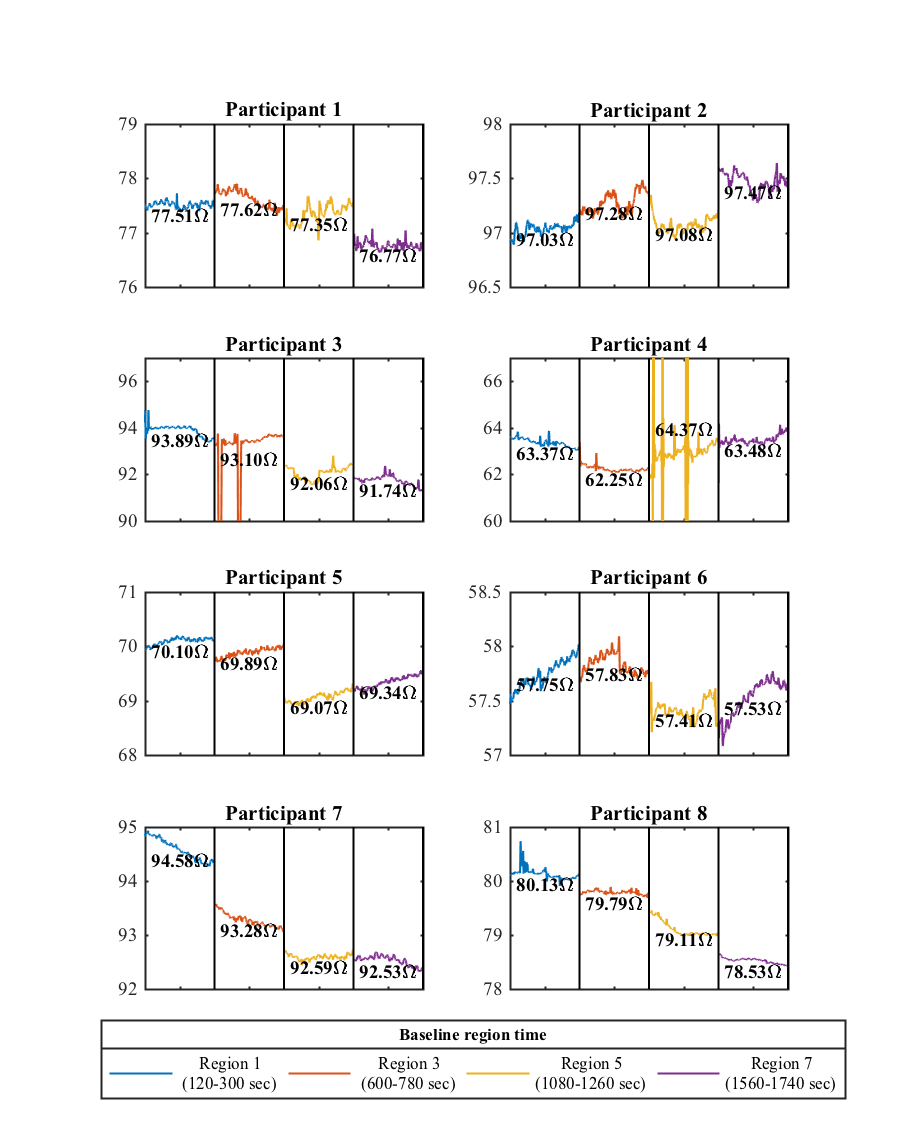
\includegraphics[width=\textwidth,keepaspectratio]{figure_b_3}    
	\caption[Measurements of the basal impedance during the whole study]{Basal impedance of all the participants during the whole study. The data collected has been divided into regions. The regions (1,3,5 and 7) in white colour represent baseline measurements. The shaded areas (regions 2,4 and 6) represent occlusive events.  }
	\label{fig:Basal Regions} 
\end{figure}

Lastly, it is evident that there are variations on the baseline impedance between regions. Also, there is not a clear trend on either the increase or decrease of the basal impedance, except on participants 7 and 8 where there is a decrease on impedance. Big gaps (< \SI{0.8}{\ohm}) between regions can be noticed on participant 5 and participant 7. It is important to determine if the change of impedance is larger than when performing VOP. Therefore, the following section analyses in depth the change of basal impedance and quantifies the changes. 

 
%%********************************** % Section 6.3.1 ******************************************
\section{Basal impedance change between regions}
\label{senction basal 3.1} 
The basal impedance signal contains noises that may deviate the signal from the baseline. As the previous section analysed, the baseline changed between baseline regions. This section will quantify the error compared to the basal impedance at the beginning of the experiment. 

Different factors could affect a bioimpedance reading. One of this is the change of impedance on the electrode-skin interface.  As described in section \ref{section impedance electrodes}, when either the geometry or the area of contact of the electrode changes, it is converted into variations in the total impedance. Also, air pockets that may form between the two elements could contribute to substantial changes in impedance.  Another contributing factor is motion artefact. In this case, the movement of the skin and muscles create different current paths. Hence, the basal impedance deviates from the baseline. 

In an in-vivo setting, it is tough to keep a participant completely motionless for the whole duration of the experiment.  During each baseline, the occlusion of the upper arm caused the participants to move and re-accommodate. Eventually, there was a change of impedance that will be analysed as follows caused by that movement and maybe a physiological response. 

The figure \ref{fig:delta percent} shows the deviation in percentage from the baseline in region 1.  Therefore, the median impedance in this region was the starting point. The data was calculated by extracting the envelope of the impedance waveform. In the figure, each point represents the median value of the resistance and the whiskers the range of the data. The oscillatory component described in the previous section caused the major variations the resistance. It can be appreciated that the baseline impedance tended to decrease in most of the participants except number 2. 

The effect of the motion artefact can be noticed on the large whiskers of some of the participants. For instance, participants 3 and 4 showed the larger ones in region 3 and 5 respectively. Indeed, the data from participant 4 was clipped as the whiskers showed a huge variation of up to \SI{200}{\percent}. It is also important to note that only a few signals were able to return to baseline. For instance, the waveforms that experienced a variation below \SI{0.25}{\percent} were the regions 3 and 4 of participant 1, participant 2 in region 5, participant 4 in region 7 and participant 6 in regions 3 and 7. The rest experience changes between \SIrange{-2.353}{0.441}{\percent} from the baseline region 1. 


\begin{figure}[!t]  %fig:rb:all_participants
	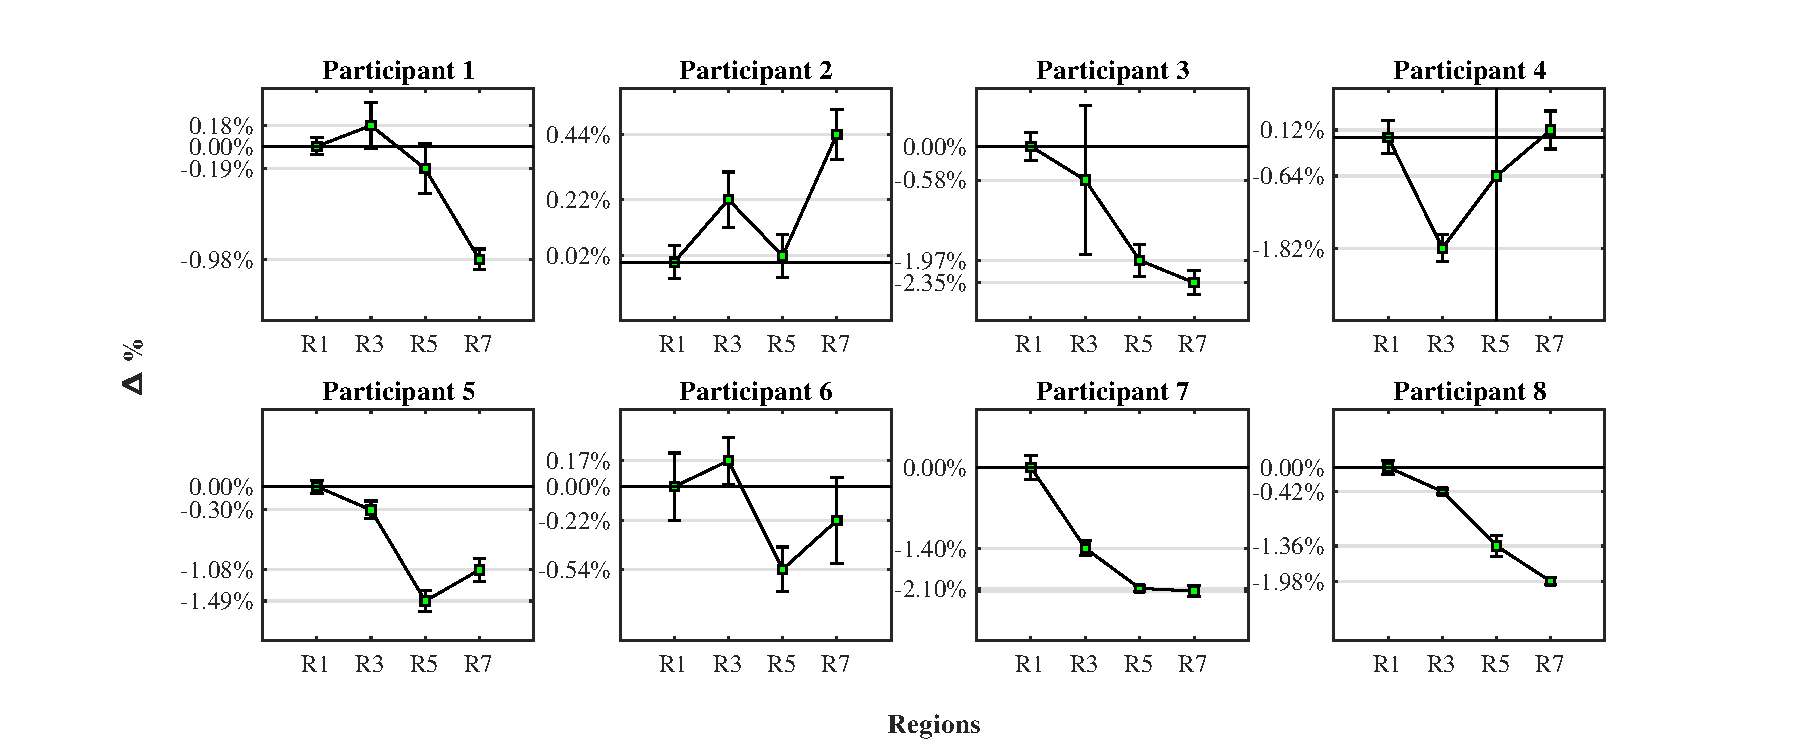
\includegraphics[width=\textwidth,keepaspectratio, trim={2cm 0cm 3cm 0cm},clip]{figure_b_4}    
	\caption[Percentil change of baseline imepdance]{Deviation of the basal impedance for all the participants compared to region 1. Each plot shows how much the impedance increase or decrease against the reference value for regions 3, 5 and 7. }
	\label{fig:delta percent} 
\end{figure}

The table \ref{tbl:change imepdance} shows the range and mean of changes of impedance for all the participants. The average impedance of the whole study was \SI{-0.6384}{\percent} with a range of about \SI{1.5264}{\percent}. Certainly, participants 1, 2 and 7 showed the least impedance change with less than \SI{0.25}{\percent}, whereas the second increased and the others decreased.  A change between \SIrange{0.25}{1}{\percent} was experienced by participants 4, 5 and 8. Finally participants 3 and 7 showed the largest change of impedance of more than \SI{1}{\percent}. 

\begin{table}[!htbp]
	\caption[Range and mean change of impedance of each participant]{Mean and range of the impedance change for each participant.}
	\label{tbl:change imepdance}
	\centering \small
	\begin{tabular}{lcc}
		\toprule
		&\textbf{range ($\Delta \%$)}
		&\textbf{mean ($\Delta \%$)} \\ \midrule
		Participant 1    &     \SI{1.157}{\percent}    &     \SI{-0.247}{\percent}    \\  
		Participant 2    &     \SI{0.441}{\percent}    &     \SI{0.170}{\percent}    \\  
		Participant 3    &     \SI{2.353}{\percent}    &     \SI{-1.226}{\percent}    \\  
		Participant 4    &     \SI{1.939}{\percent}    &     \SI{-0.584}{\percent}    \\  
		Participant 5    &     \SI{1.489}{\percent}    &     \SI{-0.719}{\percent}    \\  
		Participant 6    &     \SI{0.707}{\percent}    &     \SI{-0.148}{\percent}    \\  
		Participant 7    &     \SI{2.147}{\percent}    &     \SI{-1.412}{\percent}    \\  
		Participant 8    &     \SI{1.979}{\percent}    &     \SI{-0.940}{\percent}    \\ 
		\bottomrule 
	\end{tabular}
\end{table}

%%********************************** % Section 6.4 ******************************************
\section{Statistical analysis of basal impedance}
\label{senction basal 4} 
Identifying when the basal impedance is outside normal levels requires performing a statistical analysis. By using all the percentage deviation ($\Delta \%$) from the initial baselines as the data range, it was calculated normal probability density function (PDF). Using the Matlab command \textit{nomrfit} was computed the normal distribution from the $\Delta \%$. The calculation returned a $\mu = -0.6384$ and a $\sigma = 0.8518$. By plotting the probability distribution function can be seen how the probability distributed. Then by using the $\sigma$ obtained from the data, a new PDF was calculated centred at $\mu = 0$. As result, the PDF produces a similar data distribution where the confidence band (\SI{95}{\percent}) were calculated at $\pm 1.96 \times\sigma$.

Figure \ref{fig:basal pdf} shows the PDF obtained from the data and the new one calculated. The yellow plot shows the confidence area from the baseline. Therefore, the confidence band is between $\Delta \% = \pm 1.66 \%$. In other words, all the changes of impedance within this confidence band can be considered as statistically within normal limits. 

By comparing the results showed from the PDF calculated, most of the participants were within that range. Nevertheless, some partaker's regions are out from this confidence band. For example, regions 5 and 7 in participants 3 and 7, region 3 of participant 4 and region 7 of participant 8.

\begin{figure}[!htbp]  %fig:rb:all_participants
	\centering
	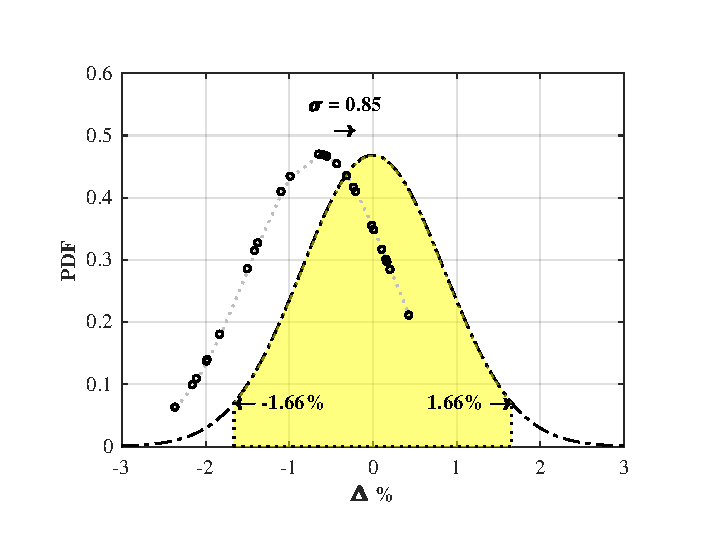
\includegraphics[width=12cm,keepaspectratio, trim={0cm 0cm 0cm 0cm},clip]{figure_b_5}    
	\caption[Percentil change of baseline imepdance]{Deviation of the basal impedance for all the participants compared to region 1. Each plot shows how much the impedance increase or decrease against the reference value for regions 3, 5 and 7. }
	\label{fig:basal pdf} 
\end{figure}

%%********************************** % Section 6.5 ******************************************
\section{Conclusion}
\label{senction basal 5} 
The basal impedance measures mostly the resistive contribution of mainly muscle, fat and skin. Also, the geometry of the segment alters the impedance reading, showing that there is an inverse relation between the volume of the segment and the average impedance. The device designed was able to take measurements within the expected ranges. However, motion artefact or the interface electrode-skin may contribute to shifting the resistance value of the measurement. The basal impedance measured was in average \SI{-0.6384}{\percent} with a maximum deviation of \SI{-2.353}{\percent}. After performing a statistical analysis of these variances, it was found that any values within $\pm 1.66 \%$ are within statistical normal values. 

%********************************** %Nomenclature found  *************************************
\nomenclature[z-pdf]{PDF}{Probability density function}